\documentclass{ximera}
\usepackage{sagetex}
%% handout
%% space
%% newpage
%% numbers
%% nooutcomes
 
%% You can put user macros here
%% However, you cannot make new environments

\graphicspath{{./}{module1Activity/}{module2Activity/}{module3Activity/}}

\usepackage{sagetex}
\usepackage{tikz}
\usepackage{hyperref}
\usepackage{tkz-euclide}
\usetkzobj{all}
\pgfplotsset{compat=1.7} % prevents compile error.

\tikzstyle geometryDiagrams=[ultra thick,color=blue!50!black]
 %% we can turn off input when making a master document
 
\outcome{}
\author{Darryl Chamberlain Jr.}
  
\title{Objective 2 - Left and Right Limits}

\begin{document}
\begin{abstract}
Interpret the notation for limits.
\end{abstract}
\maketitle
 
\href{https://cnx.org/contents/i4nRcikn@5.1:dKCfyV9u@5/The-Limit-of-a-Function}{Link to section in online textbook.}

\href{https://www.youtube.com/watch?v=7Q2HwTHcxA0}{Intro video for left/right limits.}
 
%%%%%%%%%%%%%%%%%%%%%
%%%  Objective 2  %%%
%%%%%%%%%%%%%%%%%%%%%

\Large{\textbf{Introduction to Notation}}

Let's look back at our notation: 

\begin{tabular}{l | l}
\textbf{Symbol} & \textbf{Meaning} \\
\hline 
$x \rightarrow a^{-}$ & $x$ approaches $a$ from the left \\
$x \rightarrow a^{+}$ & $x$ approaches $a$ from the right \\ 
$x \rightarrow \infty$ & $x$ approaches infinity \\ 
$x \rightarrow -\infty$ & $x$ approaches negative infinity \\ 
\end{tabular}

This gives us a way to talk about the limits of functions \textbf{when the limits on either side do not match}. Let's look back at our \href{https://www.desmos.com/calculator/x3mllngnj7}{Desmos link} of $f(x) = \frac{1}{x}$ and try to evaluate the left and right limit at $x=0$.

\begin{question}
Evaluate the following limits:	

$\lim_{x \rightarrow 0^{-}}\left( \frac{1}{x} \right) = \answer{\sage{-Infinity}}$

$\lim_{x \rightarrow 0^{+}}\left( \frac{1}{x} \right) = \answer{\sage{Infinity}}$
\end{question}

This allows us to refine our definition of a limit: 

\begin{theorem}
Relating one-sided and two-sided limits
\begin{center}

$\lim_{x \rightarrow a} (f(x)) = L$ 

if and only if 

$\lim_{x \rightarrow a^{-}} (f(x)) = L = \lim_{x \rightarrow a^{+}} (f(x))$ 
\end{center}

\end{theorem}

In other words, if the limit is equal to something, the left and right limits agree (and if the left/right limits agree, the limit is equal to something). \textit{Note: We say the limit \textbf{exists} if $L$ is a Real number. The limit can be equal to $\infty$ or $-\infty$, but we would not say the limit \textbf{exists}.}  

\Large{\textbf{Evaluating One-Sided Limits - Graphically and Analytically}}

In Calculus I, you will learn a few tricks to evaluate more difficult limits. We will focus on evaluating limits of our elementary functions: polynomials, rational, radical, logarithmic, and exponential. 

\begin{center} \textbf{Graphical Evaluation} \end{center}

When we can graph a function, it is intuitive to evaluate limits \textit{(especially limits that go to $\pm \infty$)}. We will scan along the function until we get \textit{very close} to the value we are looking at. Try to evaluate the one-sided limits below. 

\begin{question}
\[
\graph[rectangular]{f(x) = 1/x}
\]

$\lim_{x \rightarrow 0^{-}} f(x) = \answer{\sage{-Infinity}}$

$\lim_{x \rightarrow 0^{+}} f(x) = \answer{\sage{Infinity}}$

$\lim_{x \rightarrow 1^{-}} f(x) = \answer{\sage{1}}$

$\lim_{x \rightarrow {-1}^{+}} f(x) = \answer{\sage{-1}}$

\end{question}

\begin{question}
\[
\graph[rectangular]{f(x) = 1/(x-3)^2}
\]

$\lim_{x \rightarrow 3^{-}} f(x) = \answer{\sage{Infinity}}$

$\lim_{x \rightarrow 3^{+}} f(x) = \answer{\sage{Infinity}}$

$\lim_{x \rightarrow 2^{-}} f(x) = \answer{\sage{1}}$

$\lim_{x \rightarrow 2^{+}} f(x) = \answer{\sage{1}}$
\end{question}

\begin{center} \textbf{Analytical Evaluation} \end{center}

If we cannot graph a function, we may want to analytically evaluate the one-sided limit. We can do this by plugging in numbers very close to the value and see what happens with the function. 

\begin{example}
$\lim_{x \rightarrow 1^{-}} \frac{\frac{1}{x} - 1}{x - 1} = $

If we try $f(1)$, we get $\frac{0}{0}$. This doesn't help us...

Since we don't know what this graph looks like, let's try evaluating the one-sided limit analytically. We'll try the values $0.9, 0.99. 0.999, 0.9999$ \textit{since we are looking for the limit as we approach 1 from the left}.

\begin{tabular}{l|l}
	$x$ & $f(x)$ \\
	\hline 
	$0.9$ & $\answer[tolerance=0.05]{-1.11}$\\ 
	$0.99$ & $\answer{-1.01}$\\
	$0.999$ & $\answer{-1.001}$\\
	$0.9999$ & $\answer{-1.0001}$
\end{tabular}

We can keep going, but based on the chart above the limit appears to be $\answer{-1}$!

\end{example}

With technology, we can become more confident with this analytical approach. For us, this will be our best way to approximate limits of complicated functions. 

\begin{center} \textbf{Caution!} \end{center}

Limits do not care what the value is at the point!

\begin{figure}
	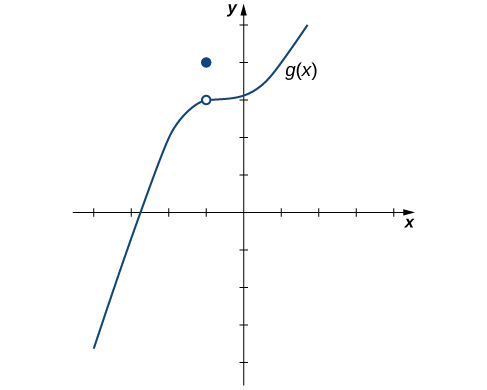
\includegraphics{CNX_Calc_Figure_02_02_006.jpg}
	\caption{\href{https://cnx.org/contents/i4nRcikn@5.1:dKCfyV9u@5/The-Limit-of-a-Function\#CNX_Calc_Figure_02_02_006}{Function with a hole at $x=-1$.}}
\end{figure}

The left- and right-sided limits of this function are both 3, so 

\begin{center} 
$\lim_{x \rightarrow -1^{+}} g(x) = 3$ \\
$\lim_{x \rightarrow -1^{-}} g(x) = 3$ \\
and \\
$\lim_{x \rightarrow -1} g(x) = 3$ \\
BUT \\
$g(-1) = 4$
\end{center}

\textbf{Practice Evaluating One-Sided Limits}

For the rest of this section, we will practice evaluating one-sided limits. You can graph these functions or use the analytical approach. 


\begin{question}
Based on the graph, evaluate the following one-sided limits.
\begin{figure}
	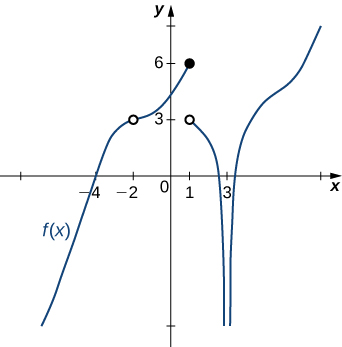
\includegraphics{CNX_Calc_Figure_02_02_015.jpg}
	\caption{\href{https://cnx.org/contents/i4nRcikn@5.1:dKCfyV9u@5/The-Limit-of-a-Function\#CNX_Calc_Figure_02_02_015}{Piecewise function to evaluate.}}
\end{figure}

$\lim_{x \rightarrow {-4}^{-}} g(x) = \answer{0}$

$\lim_{x \rightarrow {-4}^{+}} g(x) = \answer{0}$

$\lim_{x \rightarrow {-2}^{-}} g(x) = \answer{3}$

$\lim_{x \rightarrow {-2}^{+}} g(x) = \answer{3}$

$\lim_{x \rightarrow {1}^{-}} g(x) = \answer{6}$

$\lim_{x \rightarrow {1}^{+}} g(x) = \answer{3}$

$\lim_{x \rightarrow {3}^{-}} g(x) = \answer{\sage{-Infinity}}$

$\lim_{x \rightarrow {3}^{+}} g(x) = \answer{\sage{-Infinity}}$

\end{question}

\begin{question}
Let $f(x) = (1+x)^{1/x}$. Evaluate the following one-sided limits below.	

$\lim_{x \rightarrow {0}^{-}}  = \answer[tolerance=0.01]{2.7183}$

$\lim_{x \rightarrow {0}^{+}} = \answer[tolerance=0.01]{2.7183}$

$\lim_{x \rightarrow {1}^{-}}  = \answer[tolerance=0.01]{2}$
	
$\lim_{x \rightarrow {1}^{+}}  = \answer[tolerance=0.01]{2}$
\end{question}

\end{document}